% ### by András Kiss ###
% ### 2018.06.20 #######
% ### Homburg ##########


\documentclass[a4paper, 11pt]{article}
\usepackage{ae,aecompl}
\usepackage[T1]{fontenc}
\usepackage[utf8]{inputenc}
\usepackage{indentfirst}
\usepackage{xymtex}
\usepackage{multirow}
\usepackage{gensymb}
\usepackage{upgreek}
\usepackage[geometry]{ifsym}
\usepackage{subfig}
\usepackage[version=3]{mhchem}
\usepackage{float}
\usepackage{textcomp}
\frenchspacing
\usepackage[dvips]{graphicx}
\usepackage{color}
\usepackage{anysize}
\marginsize{3.2cm}{2.8cm}{3cm}{2cm}
\usepackage{enumerate}
\usepackage{cite}
\usepackage{listings}
\usepackage{setspace}
\setstretch{1.2}
\usepackage{xcolor}
\usepackage{listings}
% uncomment for hyperlinks
\usepackage[colorlinks = true,
            linkcolor = red,
            urlcolor  = blue,
            citecolor = blue,
            anchorcolor = blue]{hyperref}

\begin{document}
\thispagestyle{empty}


\thispagestyle{empty}
\begin{figure}
\centering
\includegraphics[width=0.35\textwidth, angle=-90]{8.eps}\includegraphics[width=0.35\textwidth, angle=-90]{180716_E2_8.eps}
\includegraphics[width=0.35\textwidth, angle=-90]{9.eps}\includegraphics[width=0.35\textwidth, angle=-90]{180716_E2_9.eps}
\includegraphics[width=0.35\textwidth, angle=-90]{10.eps}\includegraphics[width=0.35\textwidth, angle=-90]{180716_E2_10.eps}
\includegraphics[width=0.35\textwidth, angle=-90]{11.eps}\includegraphics[width=0.35\textwidth, angle=-90]{180716_E2_11.eps}

%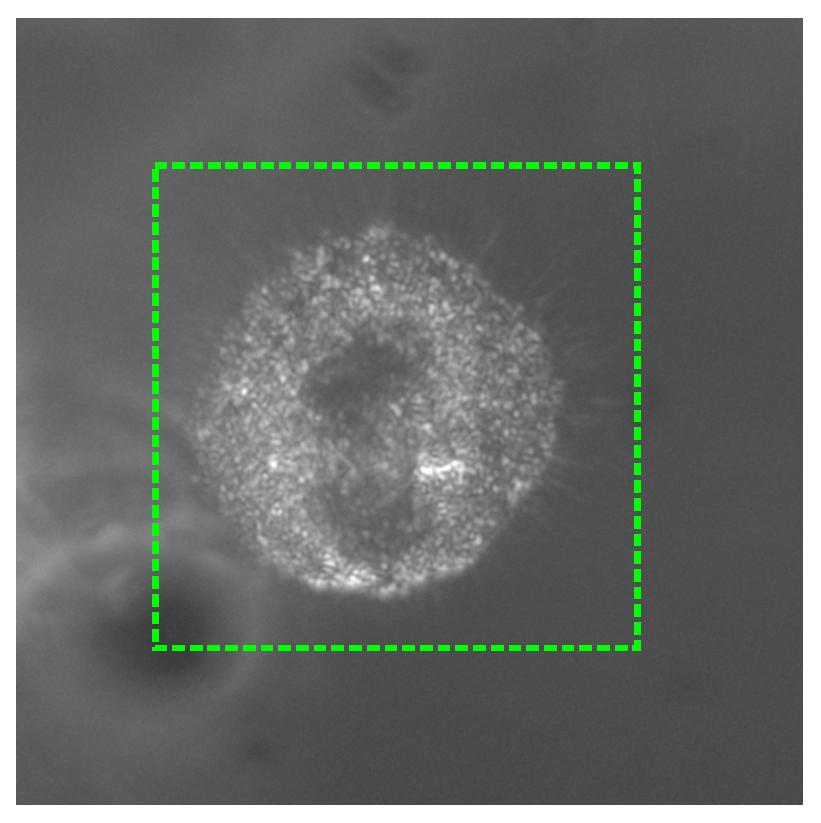
\includegraphics[width=0.40\textwidth]{monocyte_start.eps}

\caption{Oxygen reduction current above a human monocyte at h = 10 $\upmu$ relative to the glass bottom of the Petri--dish.
Working electrode: d = 10 $\upmu$m Pt UME. RG $\approx$ 2.5.
E = - 700 mV vs. Ag/AgCl quasi--refence electrode.
Medium/electrolyte: PBS + 10 mM glucose.
Date: 2018.07.16.
Left column: fixed scale -800 pA to -720 pA.
Right column: autoscale.}
\label{fig:results}
\end{figure}

\end{document}

